\chapter{Sentiment Analysis}
People's opinions, feelings and sentiments towards entities such products, services, other people, events, news, issues, topics, etc. can be in very large volume, complex and difficult to be understood and processed by machines and computers. Thus, sentiment analysis, also known as opinion mining, started to popularised along the rise of social media when large amount of digital text data were suddenly available for mining. Natural language processing (NLP) helps computers process and understand human based language to perform repetitive task. Sentiment analysis is a niche of NLP. It aims at quantifying the positivity, negativity and/or neutrality of implied or expressed in a given text.

Social media have been providing large platforms for people to share their opinion freely and expressed their views on any subject across various geographical and spatial  boundaries. They have also allowed people to connect, influence and be influenced by such opinions and views. These interactions have been studied in the 1940s and 1950s among people in organizations by management science researchers. Since 2002, with social media, those studies have been performed at grand scales with the abundance of data. Thus, advanced sentiment analysis research have been performed in field political science, economics, finance and management science as they are heavily dependent on public opinions. 

Asur and Huberman (2010) (ADD REF) attempted to solve the revenue prediction problem using both the tweet volume and the tweet sentiment. Same kind of data along with polling results were also used, in Bermingham and Smeaton (2011) (ADD REF), to train a linear regression model to predict election results. Zhang et al. (2010) (ADD REF) leveraged sentiments on Twitter to help predict the movement of stock market indices such as Dow Jones, S\&P500 and NASDAQ. It was shown that large negative emotions and opinions caused Dow to go down the next day and lower negative emotions cause Dow to go up on the next day. Bar-Haim et al. (2011) (ADD REF) on one hand leverage sentiments on Twitter but on the other did not treat all Twitter authors equally. Only expert investors were used as features in training stock price movement predictors. Undeniably, modern social media (started early 2000s) have grown into a major influencer of human opinion and sentiments.

\par 

\section{Rule-Based Methods}
Conventional NLP techniques relied on a set of rules to process textual data to extract opinion, polarity, topic, and other information within the data. Tokenization, part-of-speech tagging, lemmatization and removal of stop words are some rules and technique used to processed data prior to analysis. Tokenization is the separation/breaking down of text data into words. The space between words in a document is commonly used as the delimiter of separation. Consider the example below:
\begin{align*}
\intertext{“The price of Cryptocurrency wasn’t great today! See y’all tomorrow.”}    
\end{align*}
Tokenizing the result above results in the list:
\begin{align*}
    \intertext{“[”The”, “price”, “of”, “Bitcoin”, “was”,  “n’t”, “great”, “today”, “!”, “See”,  “y’", “all', “tomorrow”, “.”]”}    
\end{align*}
In sentiment analysis, the tokenized sentence would be compared to predefined list polarized words (positive and negative). A naive way to get the polarity of the sentence would be to count the number of positive and negative words in the predefined polarized lists. The limitations are quite obvious, we are not taking into account the context in which the words are used, nor the preceding words. Part-of-speech tagging refers to the classification of the token in a document based on predefined assignment. Tokens are classified as adjective,  adverb, noun, verb, etc. (the full list can be obtained through the universal POS tags - (ADD REF)). POS tagging is used to describe the syntactic structuring of a sentence. The part-of-speech tagging of our example in () is given by:
\begin{align*}
\intertext{*Placeholder*}   
\end{align*}
Lemmatization refers to the process of reducing words  to their base form, also known as lemma. For example, the words below can be reduced as follows:
\begin{align*}
\begin{matrix*}
    \intertext{great → good} \\
    \intertext{happiness → happy} \\
    \intertext{stemming → stem}
\end{matrix*}
\end{align*}
It allows to map the meaning of multiple words at one time by reducing the former to its base. The assumption is that both form retain the same meaning syntactically. Moreover, the removal of stop words is also often perform to eliminate words that are neutral or bring no additional value within a sentence. Examples of such word would be “the”, “a”, “is”, etc. Since rule-based models is performed individually over each word; the simple removal stop words reduced computation time of such models. However, such models are highly limited, computationally demanding and often inaccurate. Thus, with the rise of computation power available and machine learning, statistical and embedding based models were developed to tackle those limitations.
\section{Word Embedding}
Processing raw data from ruled based method is not ideal. A numerical representation of text data would be more appropriate for mathematical models to perform NLP. Word embedding is the representation of text data as vectors in a vector space. Words with similar meaning would be considered as very close to each other in such a space. Moreover, from linear algebra, we would expect that normalized vector of words with similar meaning to be close. Word embedding techniques are categorized among two types: frequency based embedding and prediction based embedding. 

Frequency based embedding refers to the vectorization of words based on the frequency of occurrence of words in a document. The three types of frequency based embedding are: Count Vector, TF-IDF (Term Frequency-Inverse Term Frequency) Vector and Co-Occurence Matrix with a fixed context window. Such type of embedding results in very sparse vector of high dimensionality which are computationally challenging to manipulate. 

Prediction based embedding refers to the prediction of a target word based on the context (neighboring words). Developed by Mikolov et al  in 2013 (ADD 2 REF), the word2vec was introduced. Word2vec is a word embedding method derived from two techniques: CBOW (Continuous Bag of Words) and Skip-Gram Model. The CBOW attempts to predict the probability of a word in the center from a given context while the Skip-Gram model is the opposite of the CBOW model; it tries to predict the context of words given a center word.
\section{Transformer Model (Attention Mechanism)}
Attention in neural network attempts to emulate the cognitive attention in the human brain. It focuses on only relevant part of the data while neglecting the rest. Developed by at team at Google Brain in 2017 \cite{Vaswani2017}, transformers are the current state-of-the-art attention techniques (instead of recurrence) for processing contextual data; text, audio, video, speech, etc. Similar to the RNN, LSTM and GRU, transformers process sequential data as well with the exception that transforms process all input at once thus allowing parallelization. Transformers consist of two main parts: the encoder and the decoder. The encoder processes the input document, identifies the important text and creates an embedding for the text based on the importance of the latter to other words in the document. The decoder on the other hand tries to get the text back from the embedding created by the encoder.
\begin{figure}[H]
    \centering
    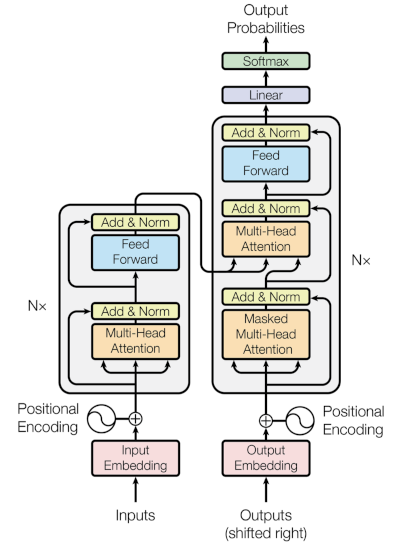
\includegraphics[scale=0.60]{CHAPTER_2/c2_fig_transformer_layer.png}
    \caption{!!!TO BE CHANGED!!!-Transformer Layer}
    \label{TRANSFORMER_LAYER}
  \end{figure}
The left part of the architecture is the encoder while the right side is the decoder. This structure allows the transformer model for parallelization computations instead of sequential (RNN, LSTM and GRU). Transformer models are now able to solve natural language processing problem with higher accuracy.  We introduce two commonly used transformation models: BERT and RoBERTa. 

Bidirectional Encoder Representations from Transformers (BERT) which was developed by Google \cite{Jacob2018}. BERT uses only the encoder part of the transformer similar to the original transformer in \cite{Vaswani2017}. 

BERT is able to create word representations that are dynamically influenced by the surrounding words, whereas word2vec has a fixed representation for each word independent of the context in which it occurs. Leading BERT to achieve multiple state-of-the-art NLP tasks when it was published, including at sentiment analysis \cite{Chiorrini2021} A number of pre-trained BERT models from unlabeled text are currently available (due to the large number of data and parameters required for training) and can be re-adapted using transfer learning. 

RoBERTa stands for Robustly Optimized BERT Pretaining Approach was also developed by Google \cite{Yinhan2019}. The approach found that BERT was currently under trained and could potentially do much better. RoBERTa uses an extensively large amount of hyperparameter, tuning and optimization. Additionally, much more data was also used during training. BERT used 16gb of data from CC-news while RoBERTa was trained on 160bg of data from CC-news (92gb), OpenWebText (38bg) and addition data from Stories (31gb) \cite{Yinhan2019}.
